\chapter{Konzeption des Prototyps}
\label{chap:konzeption}
In diesem Kapitel wird der Entwurf und die technische Konzeption des Prototyps aufbauend auf der im vorherigen Kapitel definierten Anforderungsanalyse dargelegt. Das Ziel besteht in der Entwicklung einer modularen und skalierbaren Systemarchitektur, die den gesamten Workflow von der rohen PDF-Datei bis zum strukturierten und validierten Datenexport automatisiert. Die konkrete Implementierungsdetails werden anschließend in Kapitel 6 behandelt.

\section{Systemarchitektur}
Die Architektur des Prototyps folgt dem Prinzip der Modularität und Separation of Concerns. 
Das System ist in funktional abgegrenzte Module unterteilt, die über definierte Schnittstellen miteinander kommunizieren. Diese Architektur ermöglicht eine schrittweise Entwicklung, einfache Wartbarkeit und die Möglichkeit zur späteren Erweiterung um zusätzliche Funktionalitäten \textbf{(Anforderungen FA-014, NFA-008)}. Abbildung \ref{fig:Systemarchitektur} zeigt die Gesamtarchitektur des Systems mit ihren Hauptkomponenten.

\begin{figure}[H]
    \centering
    \includegraphics[width=15cm]{images/Kapitel5/Moduldiagrammv2.png} 
    \caption{Modulare Systemarchitektur des Gleisplanextraktors}
    \label{fig:Systemarchitektur}
\end{figure}

\subsection{Dateneingabe}

Das System akzeptiert Gleispläne in verschiedenen Formaten als primäre Eingabe 
\textbf{(Anforderung NFA-010)}. Die Unterstützung mehrerer Formate berücksichtigt 
sowohl den aktuellen Anwendungsfall als auch die zukünftige Erweiterbarkeit 
auf andere Gleisplan-Layouts.

\textbf{Unterstützte Eingabeformate:}
\begin{itemize}
    \item \textbf{PDF-Dateien (.pdf):} Standardformat für technische Zeichnungen. 
    Das System rendert PDFs intern bei einer festen Auflösung von 500 DPI, was 
    eine konsistente und optimale Bildqualität gewährleistet.
    
    \item \textbf{Rastergrafiken (.png, .jpg/.jpeg, .tif/.tiff, .bmp):} Für bereits 
    rasterisierte Pläne aus Scans oder Bildexporten. Diese werden mit ihrer 
    nativen Auflösung verarbeitet.
\end{itemize}

\textbf{Auflösungsanforderung für das aktuelle Layout:}

Für das in dieser Arbeit behandelte Gleisplan-Layout ist eine Auflösung von 
exakt 500 DPI \textbf{zwingend erforderlich}. Diese strikte Anforderung ergibt 
sich aus dem Trainingsverfahren des YOLOv8-OBB Modells: Sämtliche Trainingsdaten 
wurden aus bei 500 DPI gerenderten PDFs extrahiert 
(vgl. Abschnitt~\ref{subsec:Datensatzerstellung}). Das Modell hat somit 
Pixelmuster gelernt, die spezifisch für diese Auflösung sind. Bei abweichenden 
Auflösungen, selbst bei 300 oder 400 DPI, stimmen die Symbolgrößen und 
Detailstrukturen nicht mehr mit den gelernten Mustern überein, was zu 
erheblichen Erkennungsfehlern führt.

Bei PDF-Eingaben wird die korrekte Auflösung durch die interne Rasterisierung 
automatisch sichergestellt. Bei Bilddateien muss der Benutzer gewährleisten, 
dass die Eingabe mit 500 DPI erstellt wurde. Das System zeigt einen entsprechenden 
Hinweis in der Benutzeroberfläche an.

\textbf{Erweiterbarkeit für zukünftige Layouts:}

Die Unterstützung von Bildformaten neben PDF dient primär der zukünftigen 
Erweiterbarkeit. Für neue Gleisplan-Layouts mit anderen grafischen 
Konventionen könnte ein separates YOLO-Modell mit angepasster Trainingsauflösung 
entwickelt werden. Die flexible Eingabearchitektur ermöglicht dies ohne 
Änderungen am grundlegenden Systemaufbau.

Abbildung~\ref{fig:input_processing_paths} visualisiert die differenzierte 
Behandlung der beiden Eingabepfade.

% === FIGURE: Input Processing Paths ===
\begin{figure}[H]
\centering
\begin{tikzpicture}[
    node distance=1.2cm and 2.5cm,
    font=\small,
    input/.style={rectangle, draw=blue!60!black, fill=blue!10, text width=2.8cm, 
        align=center, minimum height=1.2cm, rounded corners=3pt, thick},
    process/.style={rectangle, draw=green!60!black, fill=green!10, text width=3.2cm, 
        align=center, minimum height=1cm, rounded corners=3pt, thick},
    output/.style={rectangle, draw=orange!60!black, fill=orange!10, text width=3cm, 
        align=center, minimum height=1cm, rounded corners=3pt, thick},
    arrow/.style={->, >=Stealth, thick, draw=black!70}
]

% Input nodes
\node[input] (pdf) {PDF-Datei\\(.pdf)};
\node[input, right=3.5cm of pdf] (image) {Bilddatei\\(.png, .jpg, .tif, .bmp)};

% Processing nodes
\node[process, below=1.5cm of pdf] (render) {PyMuPDF\\Rasterisierung\\@500 DPI (fix)};
\node[process, below=1.5cm of image] (load) {Direktes Laden\\Native Auflösung\\(muss 500 DPI sein)};

% Output node
\node[output, below=1.5cm of render, xshift=2.8cm] (out) {Einheitliches\\Rasterformat\\für YOLO};

% Arrows
\draw[arrow] (pdf) -- (render);
\draw[arrow] (image) -- (load);
\draw[arrow] (render) -- (out);
\draw[arrow] (load) -- (out);

% Annotations
\node[font=\scriptsize, text width=2.5cm, align=center, below=0.05cm of render] 
    {Automatisch\\korrekt};
\node[font=\scriptsize, text width=2.5cm, align=center, below=0.05cm of load] 
    {Benutzer-\\verantwortung};

\end{tikzpicture}
\caption{Differenzierte Eingabeverarbeitung für PDF- und Bilddateien.}
\label{fig:input_processing_paths}
\end{figure}

\textbf{DPI-Konsistenz und Modellkompatibilität:}

Da das YOLOv8-OBB Modell auf Bildausschnitten trainiert wurde, die aus bei 500 DPI 
gerenderten PDFs stammen, ist die Auflösung der Eingabedaten ein kritischer Faktor 
für die Erkennungsgenauigkeit. Bei PDF-Eingaben wird dies durch die interne 
Rasterisierung automatisch sichergestellt. Bei Bilddateien liegt die Verantwortung 
für eine ausreichende Auflösung beim Benutzer. Das System zeigt daher bei 
Bildformaten einen Hinweis auf die empfohlene Mindestauflösung an:

\begin{itemize}
    \item \textbf{Optimal (500 DPI):} Volle Übereinstimmung mit Trainingsdaten, 
    maximale Erkennungsgenauigkeit
    \item \textbf{Akzeptabel (300--499 DPI):} Geringfügig reduzierte Genauigkeit, 
    für die meisten Anwendungsfälle ausreichend
    \item \textbf{Kritisch ($<$ 300 DPI):} Deutlich erhöhte Fehlerrate, nicht empfohlen
\end{itemize}

\subsection{Vorverarbeitung}
Die Vorverarbeitung transformiert die PDF Dokumente in ein für die nachfolgenden KI Module geeignetes Format. Dieser Schritt ist essentiell, weil Deep Learning basierte Objekterkennungsmodelle pixelbasierte Eingaben benötigen. Kernaufgaben des Vorverarbeitungsmoduls: 
\begin{enumerate}
    \item \textbf{Rasterisierung}: Konvertierung der PDF Seiten in hochauflösende Bilddateien (z.B. PNG, JPEG). Die Auflösung muss ausreichend hoch gewählt werden, um auch kleine Symbole und Beschriftungen erkennbar zu machen, typischerweise $\>300$ DPI.
    \item \textbf{Normalisierung}: Einheitliche Farbkanalbehandlung (z.B. Konvertierung zu Graustufen) zur Reduktion der Datenkomplexität bei gleichzeitiger Beibehaltung der relevanten visuellen Information.
    \item \textbf{Tiling (Kachelbildung)}: Große Gleispläne überschreiten häufig die maximale Eingabegröße moderner Objekterkennung (typischerweise 640x640 bis 1024x1024 Pixel). Daher wird das Gesamtbild in überlappende Ausschnitte (Tiles) unterteilt. Die Überlappung stellt sicher, dass Symbole an Kachelgrenzen nicht unvollständig erfasst werden.  
\end{enumerate}
Designentscheidungen: Die Größe der Tiles und der Überlappungsgrad sind konfigurierbare Parameter, die je nach Plandichte und Symbolgrößen angepasst werden können.


\textbf{Formatunabhängige Weiterverarbeitung:}

Unabhängig vom Eingabeformat (PDF oder Bild) sind alle nachfolgenden 
Verarbeitungsschritte (Tiling, YOLO-Inferenz, OCR und Linking) identisch. 
Dies wird durch die einheitliche Repräsentation als RGB-Array nach der 
Eingabeverarbeitung gewährleistet (vgl. Abbildung~\ref{fig:format_preprocessing} 
in Kapitel~\ref{chap:implementierung}). Die Tile-Größe von $2048 \times 2048$ Pixeln 
und der Überlappungsgrad von 12{,}5\% bleiben konstant, wobei die absolute 
Anzahl der Tiles von den Bildabmessungen und damit indirekt von der 
Eingabeauflösung abhängt.



\textbf{Differenzierte Behandlung nach Eingabeformat:}

Die Vorverarbeitung unterscheidet zwischen PDF- und Bildeingaben:

\begin{enumerate}
    \item \textbf{PDF-Eingaben:} Rasterisierung mittels PyMuPDF bei fester Auflösung 
    von 500 DPI. Die Transformationsmatrix gewährleistet eine deterministische und 
    reproduzierbare Bildqualität unabhängig von der Original-PDF-Auflösung.
    
    \item \textbf{Bildeingaben (PNG, JPEG, TIFF, BMP):} Direkte Verwendung der 
    nativen Pixeldaten ohne Reskalierung. Dies erhält die Originalqualität, 
    erfordert aber eine angemessene Eingabeauflösung durch den Benutzer. 
    Eine Hochskalierung niedrig aufgelöster Bilder wird bewusst vermieden, 
    da sie keine neuen Informationen generiert und zu Artefakten führen kann.
\end{enumerate}

Die nachfolgenden Verarbeitungsschritte (Tiling, Normalisierung) sind unabhängig 
vom Eingabeformat identisch, wodurch eine konsistente Pipeline für alle 
unterstützten Datentypen gewährleistet wird.

\subsection{Detection \& OCR}

Dieses Modul bildet das technologische Herzstück des Systems und kombiniert zwei komplementäre Erkennungsverfahren:
\begin{enumerate}
    \item \textbf{Objekterkennung} - Ein trainiertes Deep Learning Modell der YOLO Familie analysiert die vorverarbeiteten Bildausschnitte und identifiziert relevante Symbole (Signale, Weichen, GKS, etc.). Für jedes erkannte Objekt liefert das Modell:
    \begin{itemize}
        \item Die Klasse (z.B. \enquote{Signal},\enquote{Weiche})
        \item Die Bounding Box (räumliche Position im Bild)
        \item Einen Konfidenzwert (0-1), der die Sicherheit der Erkennung ergibt.
    \end{itemize}
    Die Verwendung von Oriented Bounding Boxes (OBB) ist konzeptionell vorgesehen, um rotierte Symbole präziser zu erfassen, was eine häufige Herausforderung in technischen Zeichnungen ist. 
    \item \textbf{Texterkennung} - OCR Verfahren extrahieren textuelle Informationen aus den erkannten Symbolbereichen. Die Texterkennung erfolgt räumlich fokussiert innerhalb oder in definierter Nähe der durch die Objekterkennung identifizierten Bounding Boxes. Dieser zielgerichtete Ansatz reduziert Fehler durch irrelevante Textfragmente im Gleisplan.\\
    \textbf{Konzeptionelle Herausforderung:} Text in technischen Zeichnungen kann in verschiedenen Orientierungen vorliegen. Das Konzept sieht daher eine orientierungsbewusste OCR Strategie vor, bei der Textregionen vor Erkennung normalisiert werden. 

\end{enumerate}

\subsection{Nachbearbeitung und Mapping}
Die Rohausgaben der Erkennungsmodule erfordern weitere Verarbeitungsschritte, um strukturierte und semantisch korrekte Daten zu erzeugen:
\begin{enumerate}
    \item \textbf{Datenbereinigung:} Rohe OCR Ergebnisse enthalten häufig Artefakte, Formatierungsfehler oder unerwünschte Zeichen. Regelbasierte Filter (z.B. mittels parametrischer Beziehungen) normalisieren die extrahierten Texte gemäß erwarteten Mustern.
    \item \textbf{Zusammenführung:} Die im Schritt erzeugten überlappenden Kacheln müssen wieder zu einem Gesamtbild zusammengefügt werden. Dabei werden Duplikate in den Überlappungsbereichen durch Non Maximum Suppression (NMS) eliminiert \cite{Bodla2017_SoftNMS}. 
    \item \textbf{Semantisches Mapping:} Die erkannten Symbole und Texte werden in einen semantischen Kontext überführt. Beispielsweise wird ein detektiertes Symbol der Klasse \enquote{Signal} mit dem dazugehörigen OCR Text zu einer logischen Einheit verknüpft.
\end{enumerate}
\subsection{Speicherung}
Alle extrahierten und verarbeiteten Daten werden in einem strukturierten Persistenzsystem gespeichert:\\
\textbf{Konzeptionelle Anforderungen:}
\begin{itemize}
    \item \textbf{Versionierung:} Jede Analyse eines Gleisplans erhält eine eindeutige Versions ID, um spätere Vergleiche zu ermöglichen.
    \item \textbf{Nachverfolgbarkeit:} Jedem Datensatz werden Metadaten zugeordnet(Quelldokument, Seitennummer, Koordinaten), um die Rückverfolgbarkeit zur Originalquelle zu gewährleisten.
    \item \textbf{Flexibles Schema:} Verwendung eines Datenbanksystems, das sowohl strukturierte als auch semi strukturierte Daten effizient speichern kann(z.B. PostgreSQL mit JSONB-Support)
\end{itemize}

\subsection{Benutzeroberfläche}
Die UI dient als Kontrollzentrum für alle Systemfunktionen und ermöglicht die Interaktion ohne Programmierkenntnisse:\\
\textbf{Konzeptionelle Anforderungen:}
\begin{itemize}
    \item \textbf{Prozessvisualisierung:} Anzeige des Verarbeitungsfortschritts in Echtzeit.
    \item \textbf{Ergebnisvalidierung:} Visuelle Darstellung der erkannten Objekte überlagert auf dem Original Gleisplan.
    \item \textbf{Konfigurationszugriff:} Bearbeitung von Systemparametern über intuitive Eingabemasken
    \item \textbf{Fehlerbehandlung:} Klare Fehlermeldungen und Hilfestellungen bei Problemen
\end{itemize}

\subsection{Export}
Das Exportmodul transformiert die interne Datenrepräsentation in kundengerechte Ausgabeformate:\\
\textbf{Unterstützte Formate:}
\begin{itemize}
    \item Excel(.xlsx): Strukturierte Tabellen für direkte Integration in bestehende Engineering Workflows
    \item CSV: Austauschformat für einfache Datenweiterverarbeitung
    \item JSON: Maschinenlesbares Format für API Integration in nachgelagerte Systeme
\end{itemize}

\textbf{Konzeptionelle Anforderung:} Das Exportmodul muss konfigurierbare Templates unterstützen, um unterschiedliche Kundenvorgaben für Tabellenstrukturen abzubilden.




\section{Workflow: Von PDF zu Excel}
Der zu entwickelnde Prototyp basiert auf einer klaren Struktur eines Swimlane-Diagramms mit drei Ebenen, wodurch eine saubere Trennung zwischen Benutzeroberfläche, Datenverarbeitung und Datenspeicherung gewährleistet wird. Das folgende Flussdiagramm \ref{fig:Workflowdiagramm} veranschaulicht den gesamten Prozess von der ersten Benutzereingabe bis zum endgültigen Datenexport. 
\begin{figure}[H]
    \centering
    \includegraphics[width=16cm]{images/Kapitel5/Prototyp flowchar v02.png} 
    \caption{Workflowdiagramm des Prototyps}
    \label{fig:Workflowdiagramm}
\end{figure}

\subsection{1. Ebene - UI/Frontend (Benutzeroberfläche)}

Die Frontend-Ebene bildet die Schnittstelle zwischen Anwender und System. Der konzeptionelle Ablauf umfasst:
\begin{enumerate}
    \item \textbf{Dateiauswahl:} Der Benutzer wählt eine PDF-Datei sowie optional eine Konfigurationsdatei aus
    \item \textbf{Parametereinstellung:} Konfiguration von Verarbeitungsoptionen (z.B. zu analysierende Seiten, Erkennungsmodell, OCR Engine)
    \item \textbf{Prozessinitiierung:} Start der automatisierten Analyse durch Betätigung einer \enquote{Ausführen}-Schaltfläche
    \item \textbf{Ergebnisanzeige:} Darstellung der Erkennungsergebnisse zur manuellen Überprüfung
    \item \textbf{Export:} Finalisierung und Download der aufbereiteten Daten im gewünschten Format
\end{enumerate}
Designprinzip: Der Workflow folgt einem linearen Assistenten-Modell (Wizard Pattern), das den Benutzer schrittweise durch den Prozess führt.

\subsection{2. Ebene - Backend/Verarbeitung (Kernlogik)}
Das Backend orchestriert die automatisierte Analysepipeline. Die Prozessschritte sind:

\begin{enumerate}
    \item \textbf{Rasterisierung:} Konvertierung der PDF-Seiten in Pixelbilder hoher Auflösung
    
    \item \textbf{Tiling:} Segmentierung in überlappende Bildausschnitte für effiziente Verarbeitung
    
    \item \textbf{Objekterkennung:} Detektion relevanter Symbole mittels Deep Learning Modell
    
    \item \textbf{OCR:} Extraktion von Textinformationen aus identifizierten Symbolbereichen
    
    \item \textbf{Postprocessing \& Merge:} Zusammenführung der Tile-Ergebnisse zu einem Gesamtbild und Eliminierung von Duplikaten in Überlappungsbereichen durch Non-Maximum-Suppression (NMS) \cite{Bodla2017_SoftNMS}. Rohe OCR-Ergebnisse werden durch regelbasierte Filter bereinigt.
    
    \item \textbf{Linking \& Semantisches Mapping:} Verknüpfung erkannter Symbole mit zugehörigen Texten (IDs, Koordinaten) zu logischen Einheiten. Beispielsweise wird ein detektiertes Symbol der Klasse \enquote{Signal} mit dem dazugehörigen OCR-Text zu einer semantisch interpretierbaren Entität verbunden. Die konzeptionellen Strategien hierfür werden in Abschnitt \ref{sec:linkingassociationmodul} detailliert beschrieben.
    
    \item \textbf{Validierung \& Qualitätskontrolle:} Automatisierte dreistufige Plausibilitätsprüfung der Erkennungsergebnisse auf Symbol-, OCR- und Linking-Ebene. Fehlgeschlagene Validierungen werden zur manuellen Überprüfung markiert (Human-in-the-Loop). Das vollständige Validierungskonzept ist in Abschnitt \ref{sec:validierungundqualitätssicherung} dargelegt.
    
    \item \textbf{Versionsspeicherung:} Persistierung der Ergebnisse mit Versionsmetadaten in der Datenbank. Jede Analyse erhält eine eindeutige Versions-ID, um spätere Vergleiche zu ermöglichen.
    
    \item \textbf{Exportvorbereitung:} Transformation der internen Datenrepräsentation in das gewünschte Ausgabeformat
\end{enumerate}

Designprinzip: Die Pipeline folgt dem Pipes-and-Filters Architekturmuster, bei dem jede Komponente eine spezifische Transformation durchführt und das Ergebnis an die nächste Stufe weiterreicht.

\textbf{Optionaler Versionsvergleich:} Unabhängig von der automatischen Verarbeitungspipeline kann der Benutzer über die Benutzeroberfläche einen manuellen Vergleich zwischen zwei Versionen desselben Gleisplans initiieren. Hierzu werden beide Planversionen in separaten Ansichten (Tabs) geladen. Durch Betätigung einer Vergleichsfunktion analysiert das System beide Datensätze und identifiziert Änderungen (hinzugefügte, entfernte oder modifizierte Objekte). Die konzeptionelle Vergleichsstrategie basiert auf dem in Abschnitt \ref{sec:änderungsverfolgung} beschriebenen hybriden Matching-Ansatz. Die Ergebnisse werden visuell hervorgehoben dargestellt, sodass der Benutzer Planänderungen nachvollziehen kann. Die technische Implementierung wird in Kapitel 6 beschrieben.

\subsection{3. Ebene - Speicher und Export (Datenverwaltung)}
Die unterste Ebene verwaltet die Daten des gesamten Systems, die in statischen und dynamischen Daten unterteilt sind:

\begin{itemize}
    \item \textbf{Statische Daten} umfassen die Basiskonfigurationsdaten, die die Regeln für das Mapping und die Verarbeitungsparameter definieren, sowie die trainierten Gewichte des Erkennungsmodells. Diese Daten dienen als feste Eingabeparameter für die Verarbeitung im Backend und ändern sich während der Laufzeit nicht.
    
    \item \textbf{Dynamische Daten} werden während des Verarbeitungsprozesses generiert. Zu diesem Zweck ist eine zentrale Datenbank für die dauerhafte Speicherung der Analyseergebnisse und Versionsstände erforderlich. Darüber hinaus werden temporäre Dateien wie Anzeigebilder und Overlays zwischengespeichert. Die aufbereiteten Daten werden schließlich in Form von Exportdateien bereitgestellt, die dem Nutzer zum Download zur Verfügung stehen.
\end{itemize}

Designprinzip: Die Trennung zwischen statischen und dynamischen Daten folgt dem Konzept der Immutability für Konfigurationen, während Analyseergebnisse in einem transaktionalen Datenbanksystem versioniert gespeichert werden.

\textit{Hinweis:} Die konkrete technologische Umsetzung (Datenbankschema, Dateiformate, Speicherorganisation) wird in Kapitel 6 detailliert beschrieben.

\section{Designentscheidungen}
Die Entwicklung des Prototyps erforderte fundamentale Entscheidungen bezüglich der eingesetzten Technologien und Architekturansätze. Die nachfolgenden Abschnitte dokumentieren diese Designentscheidungen mit technischer Begründung und Abgrenzung zu alternativen Lösungsansätzen.

\subsection{Datenaufbereitung: PDF-Rasterisierung mit pdf2image}
Da moderne Objekterkennungsmodelle (wie YOLO) auf Pixeldaten operieren, müssen die vektorbasierten PDF-Gleispläne in einem ersten Schritt rasterisiert werden. Hierfür wurde die Bibliothek \texttt{pdf2image} gewählt, die als Python-Wrapper für die C++-Bibliothek \textit{Poppler} fungiert.\cite{Belval2024}

Diese Komponente bildet den kritischen Eingangskanal der Pipeline. Die Entscheidung für \texttt{pdf2image} begründet sich durch folgende technische Eigenschaften:

\begin{itemize}
    \item \textbf{Rendering-Qualität (Cairo Engine):} 
    Poppler nutzt intern die \textit{Cairo}-Rendering-Engine, die eine pixelgenaue Rasterisierung von Vektorlinien und eingebetteten Textelementen gewährleistet. Für die vorliegende Arbeit wurde eine Auflösung von \textbf{500 DPI} gewählt. Diese hohe Pixeldichte ist notwendig, um filigrane Symbole (z.\,B. Weichenzungen oder Sperrsignale) auch nach der Kachelung (Tiling) noch differenzierbar für das neuronale Netz darzustellen \cite{Poppler2024}.
    
    \item \textbf{Speichereffizientes Ressourcenmanagement:} 
    Gleispläne weisen extreme Dimensionen auf (bis zu $67.000 \times 7.000$ Pixel). Ein naives Laden solcher Dateien würde den Arbeitsspeicher (RAM) handelsüblicher Workstations überlasten. \texttt{pdf2image} unterstützt eine Streaming-Verarbeitung, bei der Seiten einzeln in den Speicher geladen und sofort verarbeitet werden, ohne das Gesamtdokument im RAM zu halten.
    
    \item \textbf{Nahtlose Python-Integration:} 
    Die Bibliothek liefert die gerenderten Daten direkt als \textit{PIL}-Objekte (Python Imaging Library) zurück. Dies ermöglicht eine In-Memory-Weitergabe an den \textit{NumPy}/\textit{OpenCV}-Stack für das Preprocessing, ohne den I/O-Flaschenhals des Zwischenspeicherns auf der Festplatte \cite{Belval2024}.
\end{itemize}

\subsubsection{Abgrenzung zu alternativen Bibliotheken}
Die Auswahl wurde gegen populäre Alternativen validiert. Die folgende Tabelle fasst die Ausschlusskriterien zusammen, wobei insbesondere lizenzrechtliche Aspekte im Unternehmenskontext eine Rolle spielten:

\begin{table}[H]
    \centering
    \renewcommand{\arraystretch}{1.5}
    \begin{tabularx}{\textwidth}{|p{3.5cm}|X|}
    \hline
    \textbf{Alternative} & \textbf{Nachteil / Ausschlussgrund}\\
    \hline
    \textbf{PyMuPDF (fitz)} & \textit{Lizenzrisiko:} Obwohl PyMuPDF performant ist, unterliegt es der \textbf{AGPL-Lizenz} \cite{PyMuPDF2024}. Für eine kommerzielle Nutzung innerhalb von Siemens Mobility würde dies eine Offenlegung des gesamten Quellcodes erzwingen (Copyleft-Effekt), was für interne Tools oft ausgeschlossen ist.\\
    \hline
    \textbf{PDFminer} & \textit{Falscher Fokus:} PDFminer extrahiert die Dokumentenstruktur (Text, Metadaten), ist aber nicht in der Lage, komplexe Vektorgrafiken visuell korrekt zu rasterisieren. Für visuelle Objekterkennung ist es daher ungeeignet \cite{Shinyama2022}.\\
    \hline
    \textbf{Poppler CLI} & \textit{Systembruch:} Die direkte Nutzung der Kommandozeilen-Tools (\texttt{pdftoppm}) erfordert Systemaufrufe via \texttt{subprocess}. Dies erschwert das Exception-Handling und verhindert den direkten Datenaustausch im RAM (erzwungener File-I/O), was die Pipeline verlangsamt.\\
    \hline
    \end{tabularx}
    \caption{Vergleich verschiedener PDF-Verarbeitungsbibliotheken}
    \label{tab:Alternative_PDF}
\end{table}

Die konkrete Wahl der Rendering-Parameter (DPI-Auflösung, Farbtiefe, 
Anti-Aliasing) und die Implementierung der Pipeline wird in Abschnitt \ref{Inferenz}
(Preprocessing und Rasterisierung) beschrieben.
\subsection{Objekterkennung: Einsatz von YOLOv8 OBB}
Zur Identifizierung der schematischen Symbole (Signale, Weichen, Gleiselemente) wurde das Modell \textbf{YOLOv8} (You Only Look Once) in der spezialisierten Konfiguration für rotierte Bounding Boxes (OBB) implementiert. Diese Wahl stellt eine Abkehr von klassischen Detektoren dar und wird durch die spezifische Topologie von Gleisplänen begründet.

Die Entscheidung für YOLOv8 OBB basiert auf drei technischen Hauptfaktoren\cite{yolov8_ultralytics}:

\begin{enumerate}
    \item \textbf{Rotationsinvarianz durch OBB-Regression:} 
    Technische Gleispläne zeichnen sich durch eine hohe Dichte an Symbolen aus, die entlang der Gleisachsen in beliebigen Winkeln ($\theta \in [-90^\circ, +90^\circ]$) angeordnet sind. Herkömmliche Detektoren mit achsenparallelen Boxen (Horizontal Bounding Boxes, HBB) sind hier ungeeignet, da sie:
    \begin{itemize}
        \item Bei diagonalen Objekten (z.\,B. $45^\circ$) einen hohen Anteil an irrelevanter Hintergrundfläche einschließen (geringe Signal-to-Noise Ratio).
        \item Bei dichter Symbolfolge zu signifikanten Überlappungen (Intersection over Union, IoU) führen, was fälschlicherweise die Non-Maximum-Suppression (NMS) auslöst und benachbarte Objekte unterdrückt.
    \end{itemize}
    
    YOLOv8 OBB löst dieses Problem durch die Vorhersage eines 5-dimensionalen Vektors $(c_x, c_y, w, h, \theta)$, wobei $\theta$ den Rotationswinkel beschreibt. Dies ermöglicht eine präzise Umhüllung der Symbole unabhängig von ihrer Orientierung im Plan \cite{UltralyticsOBB}.

    \item \textbf{Echtzeitfähigkeit und Tiling-Effizienz:} 
    Da Gleispläne oft Auflösungen von über $50.000$ Pixeln Breite aufweisen, müssen sie in Hunderte kleinerer Kacheln (Tiles) zerlegt werden. Die Inferenzgeschwindigkeit ist daher kritisch für die Gesamtlaufzeit. YOLOv8 erreicht auf Standard-GPU-Instanzen (z.\,B. AWS g4dn.xlarge) eine Framerate von $\sim 40$ FPS bei einer Auflösung von $1024 \times 1024$. Dies ermöglicht die Verarbeitung eines gesamten Bahnhofsplans in wenigen Sekunden, was für eine interaktive Nutzung der Anwendung essenziell ist \cite{yolov8_ultralytics}.

    \item \textbf{Architektonische Modularität (Anchor-Free):} 
    Im Gegensatz zu älteren YOLO-Versionen nutzt v8 einen \textit{Anchor-Free}-Ansatz. Dies eliminiert die Notwendigkeit, vor dem Training manuelle Anker-Boxen basierend auf der Verteilung der Symbolgrößen zu berechnen (K-Means Clustering). Dies reduziert das Hyperparameter-Tuning erheblich und verbessert die Generalisierung auf neue, bisher unbekannte Symbolklassen \cite{10204762}.
\end{enumerate}

\subsubsection{Abgrenzung zu alternativen Detektionsverfahren}
Im Auswahlprozess wurden verschiedene Architekturen evaluiert. Die folgende Tabelle verdeutlicht, warum diese trotz spezifischer Stärken für den Anwendungsfall \enquote{Gleisplan} verworfen wurden:

\begin{table}[H]
    \centering
    \renewcommand{\arraystretch}{1.5}
    \begin{tabularx}{\textwidth}{|p{3cm}|p{4.5cm}|X|} 
    \hline
    \textbf{Alternative} & \textbf{Evaluationsergebnis} & \textbf{Grund für die Ablehnung} \\ \hline
    \textbf{RTMDet} & Hohe Präzision (mAP: 91.2\%), vergleichbar mit YOLOv8 & Obwohl die Rotation-Aware-Features vielversprechend sind, zeigte RTMDet eine instabilere Konvergenz bei kleinen Datensätzen ($<2000$ Samples) und verfügt über ein kleineres Entwickler-Ökosystem im Vergleich zu YOLO \cite{lyu2022rtmdetempiricalstudydesigning}. \\ \hline
    \textbf{Template Matching} (OpenCV) & Geringer Recall ($<60\%$) bei leichten Rotationen ($\pm 10^\circ$) & Klassische Computer-Vision-Verfahren sind nicht robust gegenüber Skalierung und Artefakten. Zudem ist der Ansatz bei $>13$ Symbolklassen rechnerisch nicht skalierbar \cite{Brunelli2009}. \\ \hline
    \textbf{DETR / DINOv2} & Trainingszeit ca. $3\times$ länger als bei CNNs & Transformer-basierte Ansätze benötigen enorme Datenmengen, um die Inductive Biases von CNNs zu lernen. Für die strukturierte Domäne technischer Zeichnungen stellt dies einen unverhältnismäßigen Ressourcenaufwand dar \cite{Carion2020_DETR}. \\ \hline
    \textbf{Faster R-CNN} & Inferenz: $\sim 8$ FPS (vs. 40 FPS bei YOLO) & Die Two-Stage-Architektur (Region Proposal Network + Classifier) ist zwar präzise, aber für das Feedback in einer User-Interface-Anwendung zu langsam \cite{Ren2015_FasterRCNN}. \\ \hline
    \end{tabularx}
    \caption{Vergleich und Bewertung von Alternativen zu YOLOv8}
    \label{tab:Alternative_Detection}
\end{table}
Die Entscheidung für YOLOv8-OBB adressiert direkt die Anforderungen \textbf{FA-001} 
(Erkennungsrate $\geq$ 90\%), \textbf{FA-002} (Rotationsinvarianz durch OBB-Regression) 
und \textbf{NFA-007} (Ressourceneffizienz durch Echtzeitfähigkeit).
\subsection{Texterkennung: Multi-Engine-Strategie und Dual-Angle-Routing}
Die Extraktion von Textinformationen aus technischen Gleisplänen stellt aufgrund variierender Schriftarten, unterschiedlicher Orientierungen ($0^\circ, 90^\circ, 270^\circ$) und der Überlagerung durch grafische Elemente eine besondere Herausforderung dar. Um eine maximale Robustheit zu gewährleisten, wurde keine einfache OCR-Lösung gewählt, sondern eine \textbf{kaskadierte Multi-Engine-Strategie} implementiert.

Das System kombiniert die Deep-Learning-basierte Bibliothek \textbf{PaddleOCR} (als Primärinstanz) mit der klassischen Engine \textbf{Tesseract} (als Fallback). Ergänzt wird dies durch einen eigens entwickelten \textbf{Dual-Angle-Routing-Algorithmus}.

\subsubsection{Primäre Engine: PaddleOCR (PP-OCRv3)}
Als Hauptkomponente kommt PaddleOCR zum Einsatz. Die Entscheidung für dieses Framework basiert auf der Architektur des PP-OCRv3-Modells, welches auf einem ultra-leichten CRNN (Convolutional Recurrent Neural Network) basiert.\cite{paddleocr} 

Die technischen Vorzüge gegenüber alternativen Engines zeigten sich in der empirischen Evaluation:
\begin{itemize}
    \item \textbf{Rotation-Robustheit:} Standard-OCR-Engines versagen oft bei vertikalem Text. PaddleOCR unterstützt zwar eine interne Klassifizierung (\texttt{use\_angle\_cls}), diese erwies sich jedoch bei kurzen technischen Bezeichnern als fehleranfällig. Daher wurde das System so konfiguriert, dass die Rotation extern durch die OBB-Koordinaten (aus dem YOLO-Schritt) vorgegeben wird, was die Stabilität signifikant erhöht \cite{du2020ppocrpracticalultralightweight}.
    
    \item \textbf{Genauigkeit (Character Error Rate - CER):} Auf einem validierten Testset von Gleisplan-Ausschnitten (Crops) erzielte PaddleOCR die niedrigsten Fehlerraten:
    \begin{itemize}
        \item \textbf{PaddleOCR:} 7.2\,\% (horizontal), 12.1\,\% (vertikal/rotiert)
        \item \textbf{Tesseract:} 11.4\,\% (horizontal), 23.8\,\% (vertikal/rotiert)
        \item \textbf{EasyOCR:} 9.1\,\% (horizontal), 18.3\,\% (vertikal/rotiert)
    \end{itemize}
    
    \item \textbf{Inferenzgeschwindigkeit:} Mit durchschnittlich \textbf{52 ms pro Crop} (CPU, 12 Threads) ist PaddleOCR deutlich effizienter als Tesseract (78 ms), was bei Plänen mit tausenden Textobjekten essentiell für die Gesamtlaufzeit ist.
\end{itemize}

\subsubsection{Algorithmus: Dual Angle Routing}
Ein neuartiger Ansatz der Pipeline ist das \textit{Dual Angle Routing}. Da die Orientierung eines Textes im CAD-Plan nicht immer eindeutig aus der Bounding Box hervorgeht (z.\,B. bei quadratischen Boxen), wird jeder Textausschnitt spekulativ in zwei Orientierungen verarbeitet:

\begin{enumerate}
    \item \textbf{Pfad A (Original):} Der Crop wird unverändert an die OCR übergeben.
    \item \textbf{Pfad B (Orthogonal):} Der Crop wird um $90^\circ$ rotiert an die OCR übergeben.
\end{enumerate}
\begin{figure}[h]
\centering
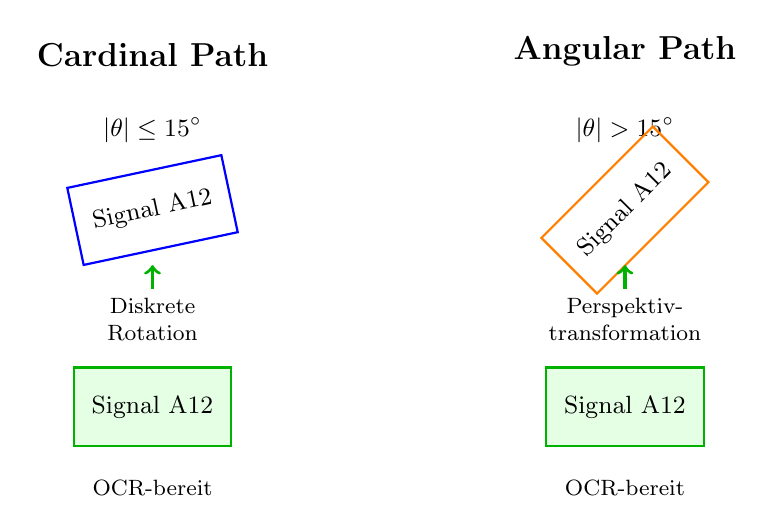
\begin{tikzpicture}[scale=1.0]
    % LEFT: Cardinal Path
    \begin{scope}
        \node[above, font=\large\bfseries] at (1.5, 3.2) {Cardinal Path};
        \node[below, font=\small] at (1.5, 2.8) {$|\theta| \leq 15^\circ$};
        
        % Slightly rotated text box (12 degrees)
        \draw[thick, blue, rotate around={12:(1.5,1.5)}] (0.5,1) rectangle (2.5,2);
        \node[rotate=12, font=\small] at (1.5,1.5) {Signal A12};
        
        % Arrow indicating transformation
        \draw[->, very thick, green!70!black] (1.5, 0.5) -- (1.5, 0.8);
        \node[below, font=\footnotesize, align=center] at (1.5, 0.5) {
            Diskrete\\Rotation
        };
        
        % Result (horizontal)
        \draw[thick, green!70!black, fill=green!10] (0.5,-1.5) rectangle (2.5,-0.5);
        \node[font=\small] at (1.5,-1) {Signal A12};
        
        \node[below, font=\footnotesize] at (1.5, -1.8) {OCR-bereit};
    \end{scope}
    
    % RIGHT: Angular Path
    \begin{scope}[xshift=6cm]
        \node[above, font=\large\bfseries] at (1.5, 3.2) {Angular Path};
        \node[below, font=\small] at (1.5, 2.8) {$|\theta| > 15^\circ$};
        
        % Heavily rotated text box (45 degrees)
        \draw[thick, orange, rotate around={45:(1.5,1.5)}] (0.5,1) rectangle (2.5,2);
        \node[rotate=45, font=\small] at (1.5,1.5) {Signal A12};
        
        % Arrow indicating transformation
        \draw[->, very thick, green!70!black] (1.5, 0.5) -- (1.5, 0.8);
        \node[below, font=\footnotesize, align=center] at (1.5, 0.5) {
            Perspektiv-\\transformation
        };
        
        % Result (horizontal)
        \draw[thick, green!70!black, fill=green!10] (0.5,-1.5) rectangle (2.5,-0.5);
        \node[font=\small] at (1.5,-1) {Signal A12};
        
        \node[below, font=\footnotesize] at (1.5, -1.8) {OCR-bereit};
    \end{scope}
\end{tikzpicture}
\caption{Konzeptioneller Vergleich der Dual-Winkel-Verarbeitungsstrategien: Cardinal Path für nahezu ausgerichtete Texte ($|\theta| \leq 15^\circ$) mit diskreter Rotation; Angular Path für stark geneigte Texte ($|\theta| > 15^\circ$) mit Perspektiventransformation}
\label{fig:dual_angle_comparison}
\end{figure}

Die Entscheidung, welches Ergebnis übernommen wird, erfolgt durch eine \textbf{Textnormierungs-Heuristik}. Beide Ergebnisse werden gegen reguläre Ausdrücke (Regex) für typische Signalbezeichnungen (z.\,B. \texttt{\^{}[A-Z]\{1,3\}[0-9]+}) geprüft. Das Ergebnis mit dem höheren Konfidenz-Score, das gleichzeitig dem Schema entspricht, wird akzeptiert. Dies eliminiert Rauschen, das entsteht, wenn vertikaler Text fälschlicherweise horizontal gelesen wird.

\subsubsection{Fallback-Ebene und Vorverarbeitung}
Für Fälle, in denen PaddleOCR keine plausiblen Ergebnisse liefert (Konfidenz $< 0.5$), greift das System auf \textbf{Tesseract 5} zurück.
\begin{itemize}
    \item \textbf{Spezialisierung:} Tesseract zeigt insbesondere bei stark pixelierten, aber hochkontrastigen Signalnamen Stärken.
    \item \textbf{Page Segmentation Modes (PSM):} Durch die explizite Setzung von \texttt{--psm 7} (Single Line) für Koordinaten und \texttt{--psm 8} (Single Word) für IDs wird die Engine gezwungen, Layout-Analysen zu überspringen, was Fehlinterpretationen reduziert \cite{Smith2007}.
    \item \textbf{Preprocessing:} Vor der OCR-Anwendung durchlaufen die Bildausschnitte eine adaptive Binarisierung nach Otsu \cite{Otsu1979gxi}, um Artefakte der PDF-Rasterung zu entfernen und den Zeichenkontrast zu maximieren.
\end{itemize}

\subsubsection{Abgrenzung zu Alternativen}
Die folgende Tabelle fasst zusammen, warum aktuelle Transformer-basierte Ansätze (\enquote{State of the Art} in der Forschung) für diesen spezifischen Anwendungsfall nicht geeignet waren:

\begin{table}[H]
    \centering
    \renewcommand{\arraystretch}{1.4}
    \begin{tabularx}{\textwidth}{|p{3.5cm}|X|}
    \hline
    \textbf{Alternative} & \textbf{Grund für den Ausschluss}\\
    \hline
    \textbf{LayoutLMv3} & \textit{Ressourcen-Overhead:} Als Transformer-Modell benötigt es GPU-Beschleunigung und ca. 2.1 GB VRAM. Für die Erkennung einzelner kurzer Textzeilen (Single-Line OCR) stellt dies einen unverhältnismäßigen Ressourcenaufwand (\enquote{Overkill}) dar \cite{huang2022layoutlmv3pretrainingdocumentai}.\\
    \hline
    \textbf{Donut (End-to-End)} & \textit{Mangelnde Generalisierung:} Da Donut (Document Understanding Transformer) direkt Bild-zu-Token generiert, ohne explizite Bounding Boxes zu nutzen, scheitert es oft an den ungewöhnlichen Vektorschriftarten der CAD-Pläne, da kein spezifisches Vortraining existiert \cite{kim2022ocrfreedocumentunderstandingtransformer}.\\
    \hline
    \textbf{TrOCR} & \textit{Rotations-Schwäche:} TrOCR ist auf horizontale Textzeilen spezialisiert. Da Gleispläne Text in beliebigen Winkeln enthalten, wäre ein komplexes Pre-Alignment notwendig, was den Vorteil der Architektur negiert \cite{li2022trocrtransformerbasedopticalcharacter}.\\
    \hline
    \end{tabularx}
    \caption{Vergleich und Bewertung alternativer OCR-Ansätze}
    \label{tab:ocr_alternatives}
\end{table}
Die Multi-Engine-Strategie mit Dual-Angle-Routing erfüllt die Anforderungen \textbf{FA-004} 
(OCR-Genauigkeit) und \textbf{FA-005} (OCR-Robustheit bei Rotation und Rauschen).
\subsection{Datenexport und Reporting: Excel Schnittstelle}
Für den Export der extrahierten Informationen und die Übergabe an die Fachabteilung wird die Funktion \texttt{pandas.DataFrame.to\_excel()} in Kombination mit der \texttt{openpyxl}-Engine verwendet. Diese Architektur ermöglicht die direkte Serialisierung der internen Datenstrukturen in das weit verbreitete \texttt{.xlsx}-Format (Office Open XML).\cite{openpyxl}

Die Entscheidung für diesen Ansatz stützt sich auf drei zentrale Gründe:

\begin{enumerate}
    \item \textbf{Feature-Vollständigkeit und Usability}: 
    Die Lösung bietet native Unterstützung für semantische Formatierungen, die die manuelle Weiterverarbeitung erleichtern:
    \begin{itemize}
        \item \textbf{Visuelle Strukturierung:} Anpassung der Spaltenbreite, Festlegen von Zellenfarben und Fixierung von Kopfzeilen (Freeze Panes).
        \item \textbf{Rückverfolgbarkeit (Traceability):} Verwendung von Formeln wie \texttt{=HYPERLINK()}, um vom Datensatz direkt auf den Bildausschnitt im Plan zu verweisen.
        \item \textbf{Multi-Sheet-Architektur:} Erstellung mehrerer Arbeitsblätter (Tabs) je nach Datenklasse (z.\,B. separate Blätter für Signale und Weichen).
    \end{itemize}
    
    \item \textbf{Integration mit pandas}: 
    Es entsteht eine nahtlose Datenfluss-Pipeline ohne Medienbruch. Die im Analyse-Schritt erzeugten DataFrames werden direkt persistiert, wobei \texttt{openpyxl} als Backend dient, um auch bestehende Templates modifizieren zu können.

    \item \textbf{Unternehmenskonformität}:
    \begin{itemize}
        \item Das \texttt{.xlsx}-Format ist der Industriestandard bei Siemens Mobility.
        \item Die Dateien sind kompatibel mit Microsoft Excel ($\geq$ 2016) und LibreOffice Calc.
        \item Da keine Makros (\texttt{.xlsm}) benötigt werden, entfallen sicherheitstechnische Hürden beim Austausch.
    \end{itemize}


    Im Rahmen der Architekturentscheidung wurden folgende Alternativen evaluiert und verworfen:

    \begin{table}[H]
        \centering
        \renewcommand{\arraystretch}{1.4} % Etwas mehr Zeilenabstand für Lesbarkeit
        \begin{tabularx}{\textwidth}{|p{3.5cm}|X|}
        \hline
        \textbf{Alternative} & \textbf{Nachteil / Ausschlussgrund}\\
        \hline
        \textbf{XlsxWriter} & Reine \textit{Write-Only}-Bibliothek \cite{XlsxWriter2024}. Sie ist zwar performant, kann aber existierende \texttt{.xlsx}-Dateien nicht einlesen oder bearbeiten, was die Nutzung von Vorlagen (Templates) verhindert.\\
        \hline
        \textbf{CSV (Textdatei)} & Keine Unterstützung für Formatierungen, Formeln oder mehrere Arbeitsblätter. Zudem bestehen Risiken durch Encoding-Probleme (UTF-8 vs. ANSI) und Trennzeichen-Konflikte.\\
        \hline
        \textbf{LibreOffice API / COM} & Systemabhängig und langsam. Erfordert eine lokale Installation der Office-Suite auf dem Server, was die Portabilität der Anwendung einschränkt.\\
        \hline
        \end{tabularx}
        \caption{Vergleich der Export-Alternativen zu pandas + openpyxl}
        \label{tab:Alternative_Export}
    \end{table}

\end{enumerate}
Die Implementierung der Export-Pipeline, einschließlich der Tabellenformatierung, 
bedingten Formatierung und Formelintegration, wird in Abschnitt \ref{subsec:exportfunktionlität}
(Excel-Export-Modul) beschrieben. Diese Architekturentscheidung erfüllt die Anforderungen \textbf{FA-009} (Excel-Integration), 
\textbf{FA-010} (Strukturerhalt bei bestehendem Template) und \textbf{NFA-012} (Ausgabeformate).
\subsection{Rückverfolgbarkeit: Koordinaten + Bildausschnitte}
Die gewählte Lösung für die Rückverfolgbarkeit ist ein hybrider Ansatz mit Koordinaten in Excel und optionaler Miniaturbildgenerierung. Für die UI-Interaktion wurde eine einfache Methode verwendet: Wird die Tabellenzeile in der Benutzeroberfläche angeklickt, so wird dem Benutzer ein vergrößerter Bereich von $2048 \times 2048$ px im Layout angezeigt, wobei die entsprechenden Datenüberlagerungen in leuchtendem Rot hervorgehoben sind.\\
Die Gründe für diese gewählte Lösung sind:
\begin{itemize}
    \item Kompaktheit: Die Koordinaten benötigen nur 8 Byte und 50 KB pro Miniaturansicht, was einen sehr geringen Speicherplatzbedarf darstellt und eine sehr hohe Funktionalität bieten. 
    \item Flexibilität: Auf Wunsch des Benutzers kann die Benutzeroberfläche den entsprechenden vergrößerten Bereich für eine genauere und präzisere Analyse darstellen. 
    \item Normkonformität: Diese Methode erfüllt außerdem die Anforderungen der VDI 1000:2017-06 hinsichtlich Rückverfolgbarkeit.\cite{VDI1000} 
\end{itemize} 
Andere Alternative
\begin{table}[H]
\centering
\renewcommand{\arraystretch}{1.3} % More row height
\begin{tabularx}{\textwidth}{|p{4cm}|X|}
\hline
\textbf{Alternative} & \textbf{Nachteil}\\
\hline
\textbf{Nur Bildausschnitte} & Datenmenge: ~12 MB für 250 Symbole; keine maschinelle Weiterverarbeitung\\
\hline
\textbf{Nur Hyperlinks} & Externe PDF-Abhängigkeit; kein Inline-Preview in UI\\
\hline
\textbf{Bildoverlay in Excel} & Excel Dateigröße >100 MB; Leistungsprobleme
\\
\hline
\end{tabularx}
\caption{Alternativen zu pandas + openpyxl}
\label{tab:Alternative5}
\end{table}
\subsection{Änderungsverfolgung: Konzeptioneller Ansatz}
\label{sec:änderungsverfolgung}
Das System unterstützt die Versionierung von Gleisplänen, um Änderungen zwischen 
verschiedenen Planständen nachvollziehbar zu machen.

\subsubsection{Konzeptionelle Strategie}

Die Änderungserkennung basiert auf einem zweistufigen Vergleichsansatz:

\begin{enumerate}
  \item \textbf{Objektidentifikation}: Jedes extrahierte Symbol erhält eine eindeutige 
        Kennung (UID), die aus Objektklasse und Textinhalt gebildet wird. Dies ermöglicht 
        die eindeutige Zuordnung zwischen Planversionen.
        
        Beispiel: Ein Signal mit der Bezeichnung \enquote{AS102} erhält die UID \texttt{signal\_AS102}.
  
  \item \textbf{Differenzbildung}: Durch Mengenoperationen auf den UID-Mengen werden 
        Änderungen kategorisiert:
        \begin{itemize}
          \item \textbf{Hinzugefügt}: Objekte, die nur in der neuen Version existieren
          \item \textbf{Entfernt}: Objekte, die nur in der alten Version existieren
          \item \textbf{Modifiziert}: Objekte mit gleicher UID, aber unterschiedlichen 
                Attributen (Position, Text)
        \end{itemize}
\end{enumerate}

\subsubsection{Hybrid-Matching für Positionsänderungen}

Wenn ein Symbol räumlich verschoben wurde, kann die UID-basierte Zuordnung versagen. 
Daher wird ein Hybrid-Ansatz verwendet:

\begin{itemize}
  \item \textbf{Primär}: Räumlicher Abgleich über OBB-Überlappung (IoU)
  \item \textbf{Fallback}: Textbasierter Abgleich über Ähnlichkeitsmetriken
\end{itemize}

Die Ergebnisse werden als strukturierter Änderungsbericht exportiert, der die Art der 
Änderung, die betroffenen Attribute und die Positionen dokumentiert.

Die technische Implementierung dieser Strategie, einschließlich der mathematischen 
Formulierung und der Algorithmen, wird in Abschnitt \ref{subsec:vergleichundänderung} detailliert beschrieben.

\subsection{Benutzeroberfläche: PyQt5}
Für die Benutzeroberfläche wurde das Framework PyQt5 aus der Python-Bibliothek ausgewählt. Die Gründe für diese Wahl werden nachfolgend dargelegt\cite{pyqt5}:
\begin{enumerate}
    \item Leistung und Rendering Architektur - Die Kernaufgabe der Anwendung ist die Visualisierung von extrem hochauflösenden Gleisplänen (bis zu 67.000 x 7.000 Pixel).
    \begin{itemize}
        \item Hardwarebeschleunigung: PyQt5 nutzt über die QGraphicsView-Klasse direkt die OpenGL-Schnittstelle der Grafikkarte. Dies ermöglicht eine Hardwarebeschleunigung für Zoomen und Schwenken ohne Ruckeln.
        \item Multithreading: Um das Blockieren der Benutzeroberfläche (UI Freezing) während rechenintensiver Operationen (YOLO-Inferenz, OCR-Verarbeitung) zu verhindern, wurde eine asynchrone Architektur mittels QThread und dem Signal-Slot-Mechanismus implementiert. Dies garantiert, dass die GUI auch während der Analyse reaktionsfähig bleibt.
    \end{itemize}
    \item Unternehmenssicherheit und Datensouveränität: Im Zusammenhang mit kritischer Eisenbahninfrastruktur ist der Schutz vertrauenswürdiger Gleisplanungsdaten von höchster Priorität:
    \begin{itemize}
        \item On-Premise Deployment: Die Anwendung läuft vollständig lokal auf dem Rechner des Ingenieurs. Es findet keine Datenübertragung an externe Server oder Cloud-Dienste statt.
        \item Security by Design: Durch den Verzicht auf Browser-Technologien entfallen typische Web-Angriffsvektoren wie Cross-Site Scripting (XSS) oder unerwünschtes Data-Leakage durch Browser-Extensions. Die Datenhoheit bleibt im lokalen Dateisystem.
    \end{itemize}
    \item Ergonomie und Multi-Monitor-Workflows: PyQt5 zeichnet sich durch eine hohe Flexibilität in der Fensterverwaltung aus. Ingenieure nutzen in vielen Fällen mehrere Monitore, um den Gleisplan auf einem Bildschirm und die tabellarischen Daten auf dem anderen Bildschirm zur Überprüfung anzuzeigen. Mittels dieses Frameworks ist es möglich, die Fenster derart zu arrangieren, dass die Daten im Gleisplan effizient aufgefunden und überprüft werden können. Diese Lösung ermöglicht zudem das dynamische Ausklappen (Popping out) von Widgets. Dies trägt zur Ergonomie bei und reduziert den Zeit- und Arbeitsaufwand beim Wechseln zwischen Fenstern oder Registerkarten. 
    \item Vergleich mit alternativen Technologien: Im Vorfeld der Entwicklung wurden verschiedene UI-Frameworks evaluiert. Die folgende Tabelle fasst die Gründe für deren Ausschluss zusammen:
    \begin{table}[ht]
    \centering
    \begin{tabular}{|p{2.5cm}|p{4cm}|p{9cm}|} 
        \hline
        \textbf{Alternative} & \textbf{Technologie} & \textbf{Hauptgrund für den Ausschluss} \\ \hline
        Streamlit & Python Web-Wrapper & Kein Multi-Window Support- Statelessness erzwingt ständiges Neuladen (Rerun) bei Interaktionen, was bei großen Bildern zu inakzeptablen Wartezeiten führt.\cite{StreamlitSecurity} \\ \hline
        Flask / Django & Web Backend & Overhead \& Komplexität \cite{Flask2024}- Erfordert lokalen Webserver und Browser; keine native Integration in das Dateisystem (Drag \& Drop, native Dialoge).\\ \hline
        Electron & JS/Chromium & Ressourcenverbrauch \cite{Electron2024}- Hoher Speicherbedarf durch gebündelte Chromium Instanz; Sicherheitsrisiken durch JavaScript Bibliotheken; Performance bei 60k Pixel Bildern unterlegen.\\ \hline
        Tkinter & Python Native & Veraltete UX \cite{Tkinter2024}; Fehlende GPU-Beschleunigung für Canvas-Elemente; keine moderne HiDPI-Skalierung (\enquote{blurry} Text auf 4K-Monitoren).\\ \hline
    \end{tabular}
    \caption{Alternative zu PyQt5}
    \label{tab:Alternative6}
    \end{table}
Die Wahl von PyQt5 als Desktop-Framework adressiert die Anforderungen \textbf{FA-013} 
(GUI ohne CLI-Kenntnisse), \textbf{NFA-001} (On-Premise-Verarbeitung ohne Cloud) und 
\textbf{FA-012} (visuelle Validierung durch Overlay-System).
\subsection{Datenpersistenz und Speicherschicht: PostgreSQL}
Für die dauerhafte Speicherung der Analyseergebnisse und Gleisplandaten wurde das objekt-relationale Datenbanksystem (ORDBMS) PostgreSQL gewählt. Die Implementierung verfolgt einen hybriden Ansatz (\enquote{Relational + Document Store}), der die Transaktionssicherheit einer SQL-Datenbank mit der Flexibilität einer dokumentenorientierten Speicherung (via JSONB) kombiniert.\cite{postgresql_docs}
\begin{enumerate}
    \item Schema-Design und Datenspeicherung: Das zentrale Speicherelement ist die Tabelle \textit{workspaces}. Anstatt für jede erkannte Objektklasse (Signale, Weichen, Texte) separate relationale Tabellen anzulegen, werden die heterogenen Analyseergebnisse in einem semi-strukturierten Format aggregiert. Dieser Entwurf adressiert zwei spezifische Anforderungen der Gleisplananalyse:
    \begin{itemize}
        \item Semi strukturierte Metadaten(JSONB): Die Ergebnisse der Objekterkennung (Bounding Boxes, Klassenwahrscheinlichkeiten, OCR-Texte) variieren stark in ihrer Struktur. Das JSONB-Format (Binary JSON) erlaubt es, diese hierarchischen Daten effizient zu speichern, ohne das Datenbankschema bei jeder Änderung der YOLO-Klassen anpassen zu müssen (Schema Evolution). Der GIN-Index (Generalized Inverted Index) ermöglicht dabei Abfragen auf tief verschachtelte Attribute (z. B. \enquote{Finde alle Pläne mit Signalen vom Typ AH}) in logarithmischer Zeit, vergleichbar mit klassischen Spaltenindizes.
        \item Binäre Topologie-Daten (BYTEA): Das extrahierte Gleisskelett (der Graph der Fahrwege) liegt zur Laufzeit als speicheroptimiertes NumPy-Array vor. Die Konvertierung in Textform (JSON/CSV) wäre ineffizient und würde Präzision kosten. Daher wird dieses Array direkt als binäres Objekt (BYTEA) persistiert, was Ladezeiten minimiert und die exakte Repräsentation der Gleisgeometrie wahrt.
    \end{itemize}
    \item Versionierung und \enquote{Upsert}-Strategie: Um Dateninkonsistenzen bei mehrfacher Analyse desselben Plans zu vermeiden, implementiert die Anwendung eine UPSERT-Logik (Update or Insert)
    \item Vorbereitung für Active Learning (Human in the Loop): Ein wesentliches Ziel der Architektur ist die nachhaltige Verbesserung der KI Modelle durch Nutzer Feedback (siehe Kapitel 8.3.2). Hierfür wurde ein separates Schema entworfen, das Abweichungen zwischen KI-Vorhersage und Nutzerkorrektur protokolliert:
    \item Abgrenzung zu alternativen Speichertechnologien
        \begin{table}[ht]
    \centering
    \begin{tabular}{|p{2cm}|p{4cm}|p{8.5cm}|} 
        \hline
        \textbf{Alternative} & \textbf{Evaluationsergebnis} & \textbf{Begründung der Ablehnung} \\ \hline
        SQLite & Bedingt geeignet & Obwohl leichtgewichtig, fehlt SQLite eine robuste Multi-User-Unterstützung (Database Locking bei Schreibzugriffen) und die JSON-Abfragefunktionen sind weniger performant als die GIN-Indizierung von PostgreSQL.\cite{SQLiteVsPostgres} \\ \hline
        MongoDB & Nicht gewählt & Als native NoSQL-DB wäre sie für JSON gut geeignet \cite{MongoDB2024}, bietet jedoch schwächere Garantien für relationale Integrität (z. B. Foreign Keys für user\_corrections) und erhöht die Komplexität im Deployment (zusätzliche Infrastruktur-Komponente).\\ \hline
        JSON-Files & Ungenügend & Die Speicherung in reinen Textdateien bietet keine Transaktionssicherheit (ACID), keine Indizierung für schnelle Suchen und führt bei parallelen Zugriffen zu \enquote{Race Conditions}.\\ \hline
    \end{tabular}
    \caption{Alternativen zu PostgreSQL}
    \label{tab:Alternative7}
    \end{table}
\end{enumerate}





\end{enumerate}
Das Datenbankdesign unterstützt die Anforderungen \textbf{NFA-005} (Prüfbarkeit durch 
Metadaten-Persistierung), \textbf{FA-011} (Änderungsverfolgung durch Versionierung) und \textbf{NFA-002} (Lizenzkonformität durch Open-Source-Datenbank).
\section{Linking- \& Assoziationsmodul}
\label{sec:linkingassociationmodul}
Die semantische Interpretation der Gleispläne erfordert die korrekte Verknüpfung 
zwischen erkannten Symbolen (Ankerobjekten) und den zugehörigen Texten (IDs, Koordinaten). 
Dieses Modul adressiert die Anforderungen \textbf{FA-006} (Fahrtrichtungsdetektion) und 
\textbf{FA-007} (Symbol-Koordinaten-Verknüpfung).

\subsection{Konzeptioneller Ansatz}

Das Linking-Modul basiert auf drei Kernprinzipien:

\begin{enumerate}
  \item \textbf{Rotationsinvariante Geometrie}: 
  Räumliche Beziehungen (z.B. \enquote{Text befindet sich unterhalb des Symbols}) werden 
  im lokalen Koordinatensystem der OBB bewertet, nicht im globalen Bildkoordinatensystem. 
  Dies gewährleistet robuste Verknüpfungen unabhängig von der Symbolorientierung.
  
  \item \textbf{Klassenspezifische Regeln}: 
  Für jede Objektklasse sind typische Text-Positionen definiert (z.B. Signalbezeichnungen 
  oberhalb des Symbols, Koordinaten unterhalb). Diese Regeln basieren auf Domänenwissen 
  über Gleisplan-Konventionen.
  
  \item \textbf{Adaptive Mustererkennung}: 
  Das System lernt wiederkehrende Layoutmuster aus erfolgreichen Verknüpfungen und 
  nutzt diese zur Verbesserung zukünftiger Zuordnungen (vgl. Abschnitt \ref{subsec:adaptivelearningmechanism}).
\end{enumerate}

\subsection{Verknüpfungsstrategien}

\subsubsection{Proximity-basierte Suche}

Textkandidaten werden innerhalb klassenspezifischer Suchradien um das Ankersymbol 
gesucht. Die Auswahl erfolgt nach:

\begin{itemize}
  \item Minimaler euklidischer Distanz
  \item Richtungskonformität (z.B. \enquote{unterhalb} für Koordinaten)
  \item OCR-Konfidenz bei mehreren Kandidaten
\end{itemize}

\subsubsection{Speziallogiken}

Für komplexe Entitäten wurden spezialisierte Verknüpfungsalgorithmen entwickelt:

\begin{itemize}
  \item \textbf{Fahrtrichtungserkennung}: Geometrische Ableitung aus der relativen 
        Position von Signal und Gleiskoppelspule(festkodiert)
  \item \textbf{Haltepunkt-Gruppierung}: Kollinearitätstest zur Verknüpfung von 
        Haltepunkt-Symbol, Signal und Koordinate
\end{itemize}

Die mathematische Formulierung und algorithmischen Details werden im Abschnitt \ref{sec:intelligentesymboltextverknüpfung} dargelegt.

\section{Validierung und Qualitätssicherung}
\label{sec:validierungundqualitätssicherung}
Das Validierungskonzept adressiert die Anforderungen \textbf{FA-008} (manuelle Korrektur durch Human-in-the-Loop), \textbf{NFA-004} (Robustheit durch Fehlerbehandlung) und 
\textbf{NFA-005} (Prüfbarkeit durch strukturierte Validierungsberichte).Das Validierungskonzept gliedert sich in drei Ebenen:

\begin{enumerate}
    \item \textbf{Symbolvalidierung}: Prüfung erkannter Objekte gegen erwartete 
    Bounding-Box-Geometrien (Größe, Seitenverhältnis, Kompaktheit).
    
    \item \textbf{OCR-Validierung}: Regex-basierter Abgleich extrahierter Texte 
    mit domänenspezifischen Mustern (Signal: \texttt{[A-Z]\{1,4\}\textbackslash d\{1,4\}}, 
    Koordinate: \texttt{\textbackslash d+[.,]\textbackslash d+}).
    
    \item \textbf{Linking-Validierung}: Plausibilitätsprüfung räumlicher Assoziationen 
    (Distanzschwellenwerte, Richtungskonformität).
\end{enumerate}

Fehlgeschlagene Validierungen werden zur manuellen Prüfung markiert (Human-in-the-Loop). 
Implementierung in Kapitel 6.5.
